\documentclass{article}\usepackage[]{graphicx}\usepackage[]{color}
%% maxwidth is the original width if it is less than linewidth
%% otherwise use linewidth (to make sure the graphics do not exceed the margin)
\makeatletter
\def\maxwidth{ %
  \ifdim\Gin@nat@width>\linewidth
    \linewidth
  \else
    \Gin@nat@width
  \fi
}
\makeatother

\definecolor{fgcolor}{rgb}{0.345, 0.345, 0.345}
\newcommand{\hlnum}[1]{\textcolor[rgb]{0.686,0.059,0.569}{#1}}%
\newcommand{\hlstr}[1]{\textcolor[rgb]{0.192,0.494,0.8}{#1}}%
\newcommand{\hlcom}[1]{\textcolor[rgb]{0.678,0.584,0.686}{\textit{#1}}}%
\newcommand{\hlopt}[1]{\textcolor[rgb]{0,0,0}{#1}}%
\newcommand{\hlstd}[1]{\textcolor[rgb]{0.345,0.345,0.345}{#1}}%
\newcommand{\hlkwa}[1]{\textcolor[rgb]{0.161,0.373,0.58}{\textbf{#1}}}%
\newcommand{\hlkwb}[1]{\textcolor[rgb]{0.69,0.353,0.396}{#1}}%
\newcommand{\hlkwc}[1]{\textcolor[rgb]{0.333,0.667,0.333}{#1}}%
\newcommand{\hlkwd}[1]{\textcolor[rgb]{0.737,0.353,0.396}{\textbf{#1}}}%
\let\hlipl\hlkwb

\usepackage{framed}
\makeatletter
\newenvironment{kframe}{%
 \def\at@end@of@kframe{}%
 \ifinner\ifhmode%
  \def\at@end@of@kframe{\end{minipage}}%
  \begin{minipage}{\columnwidth}%
 \fi\fi%
 \def\FrameCommand##1{\hskip\@totalleftmargin \hskip-\fboxsep
 \colorbox{shadecolor}{##1}\hskip-\fboxsep
     % There is no \\@totalrightmargin, so:
     \hskip-\linewidth \hskip-\@totalleftmargin \hskip\columnwidth}%
 \MakeFramed {\advance\hsize-\width
   \@totalleftmargin\z@ \linewidth\hsize
   \@setminipage}}%
 {\par\unskip\endMakeFramed%
 \at@end@of@kframe}
\makeatother

\definecolor{shadecolor}{rgb}{.97, .97, .97}
\definecolor{messagecolor}{rgb}{0, 0, 0}
\definecolor{warningcolor}{rgb}{1, 0, 1}
\definecolor{errorcolor}{rgb}{1, 0, 0}
\newenvironment{knitrout}{}{} % an empty environment to be redefined in TeX

\usepackage{alltt}
\usepackage{multirow}
\setlength\parindent{0pt}
\usepackage{geometry}
\usepackage{longtable}
\usepackage{float}
\geometry{left=1.5cm,right=1.5cm,top=1.5cm,bottom=1.5cm}

\title{Catagorical Data Analysis HW2}
\author{Faizan Khalid Mohsin}
\IfFileExists{upquote.sty}{\usepackage{upquote}}{}
\begin{document}
\maketitle






\section*{Question 1}
Describe the rationale for accommodating excess zeros in the model. Cover
both how these data indicate the necessity for such accommodation and why
this indication should not be ignored. [8 points]

\vspace{5mm}

{\bf Answer:} First, we plot the histogram of the number of drinks consumed by the participantS over the past 24 hours. 

\begin{knitrout}
\definecolor{shadecolor}{rgb}{0.969, 0.969, 0.969}\color{fgcolor}\begin{kframe}
\begin{alltt}
\hlstd{daata} \hlkwb{=} \hlkwd{read.csv}\hlstd{(}\hlstr{"assignment2_data.csv"}\hlstd{)}

\hlkwd{qplot}\hlstd{(etoh,} \hlkwc{data}\hlstd{=daata,} \hlkwc{geom}\hlstd{=}\hlstr{"histogram"}\hlstd{,} \hlkwc{main} \hlstd{=} \hlstr{"Histogram of drinks consumed by participants in the last 24 hours"}\hlstd{)}
\end{alltt}
\end{kframe}

{\centering 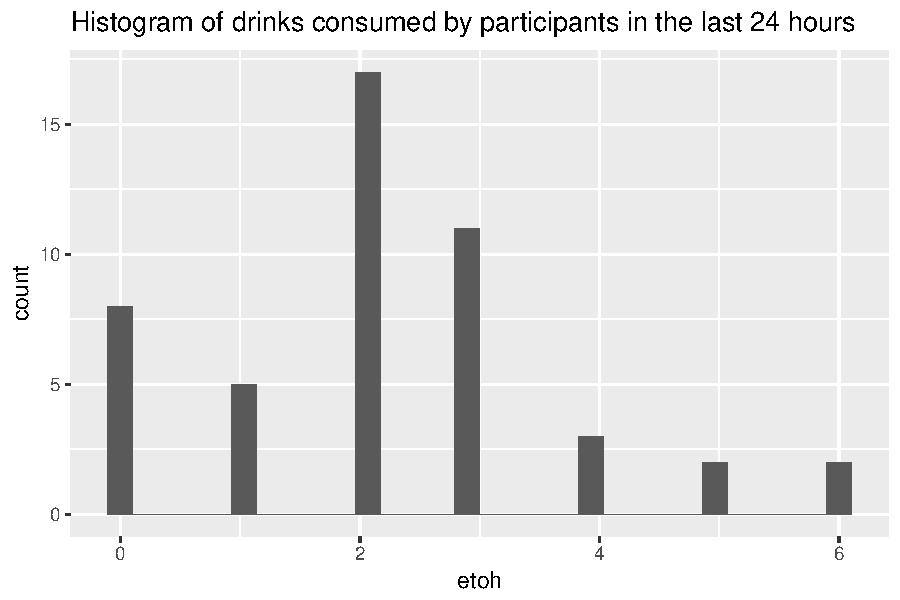
\includegraphics[width=\maxwidth]{figure/unnamed-chunk-2-1} 

}



\end{knitrout}

We can see that at zero there is a sudden spike as well as at 2. Apart from this two particular spikes the distribution of the number of drinks consumed by the participants over the past 24 hours looks more or less like the poisson distribution (of a poisson count data). Hence, this would suggest one to model the data as poisson ditribution. However, the spike seems to contain some information about something unique happening at zero, i.e. a lot more people are not drinking any alchohol in the last 24 hours than expected. Hence, we would like to incorporate this feature of the data into our model so that our model fits the data better and is able to give more informative analysis  (information) and insight and shed more light on the matter to examine patient characteristics associated with self-medication through alcohol consumption.

\vspace{5mm}

We now fit a poisson distribution to show how well such a distribution fits the data. 

\begin{knitrout}
\definecolor{shadecolor}{rgb}{0.969, 0.969, 0.969}\color{fgcolor}\begin{kframe}
\begin{alltt}
\hlcom{# # Fitting the poisson regression:}
\hlcom{# }
\hlcom{# summary(m1 <- glm(etoh ~ hx + ptsdsx + affect, family="poisson", data=daata))}
\hlcom{# }
\hlcom{# # Estimating the counts:}
\hlcom{# }
\hlcom{# pois_counts1 = predict(m1, daata, type="response", se.fit=TRUE)$fit}


\hlcom{# estimating the poisson parameter lambda from the data}
\hlstd{parms} \hlkwb{<-} \hlkwd{fitdistr}\hlstd{(daata}\hlopt{$}\hlstd{etoh,} \hlstr{"poisson"}\hlstd{)}
\hlstd{parms}
\end{alltt}
\begin{verbatim}
##     lambda  
##   2.2083333 
##  (0.2144923)
\end{verbatim}
\begin{alltt}
\hlstd{lambda} \hlkwb{<-} \hlstd{parms}\hlopt{$}\hlstd{estimate}
\hlstd{lambda}
\end{alltt}
\begin{verbatim}
##   lambda 
## 2.208333
\end{verbatim}
\begin{alltt}
\hlcom{# producing the poisson counts using the estimated lambda}
\hlstd{n} \hlkwb{=} \hlkwd{sum}\hlstd{(}\hlkwd{c}\hlstd{(}\hlnum{8}\hlstd{,}\hlnum{5}\hlstd{,}\hlnum{17}\hlstd{,}\hlnum{11}\hlstd{,}\hlnum{3}\hlstd{,}\hlnum{2}\hlstd{,}\hlnum{2}\hlstd{))}

\hlstd{poisson_counts} \hlkwb{=} \hlkwd{round}\hlstd{(n}\hlopt{*}\hlkwd{dpois}\hlstd{(}\hlnum{0}\hlopt{:}\hlnum{6}\hlstd{, lambda),} \hlnum{0}\hlstd{)}

\hlkwd{rbind}\hlstd{(}\hlkwd{c}\hlstd{(}\hlnum{0}\hlstd{,}\hlnum{1}\hlstd{,}\hlnum{2}\hlstd{,}\hlnum{3}\hlstd{,}\hlnum{4}\hlstd{,}\hlnum{5}\hlstd{,}\hlnum{6}\hlstd{), poisson_counts)}
\end{alltt}
\begin{verbatim}
##                [,1] [,2] [,3] [,4] [,5] [,6] [,7]
##                   0    1    2    3    4    5    6
## poisson_counts    5   12   13    9    5    2    1
\end{verbatim}
\begin{alltt}
\hlstd{a} \hlkwb{=} \hlkwd{as.character}\hlstd{(}\hlnum{0}\hlopt{:}\hlnum{6}\hlstd{)}
\hlstd{data} \hlkwb{=} \hlkwd{data.frame}\hlstd{(}\hlkwc{etoh} \hlstd{= a,}  \hlkwc{actual_counts} \hlstd{=} \hlkwd{c}\hlstd{(}\hlnum{8}\hlstd{,}\hlnum{5}\hlstd{,}\hlnum{17}\hlstd{,}\hlnum{11}\hlstd{,}\hlnum{3}\hlstd{,}\hlnum{2}\hlstd{,}\hlnum{2}\hlstd{),} \hlkwc{poisson_counts} \hlstd{= poisson_counts)}

\hlcom{# Producing the Histrogram of the two counts side by side. }
\hlstd{datta} \hlkwb{=} \hlkwd{melt}\hlstd{(data)}

\hlkwd{names}\hlstd{(datta)[}\hlnum{3}\hlstd{]} \hlkwb{<-} \hlstr{"counts"}

\hlkwd{ggplot}\hlstd{(datta,} \hlkwd{aes}\hlstd{(etoh,counts,} \hlkwc{fill} \hlstd{= variable),} \hlkwc{xlab}\hlstd{=}\hlstr{"etoh"}\hlstd{)} \hlopt{+}
\hlkwd{geom_bar}\hlstd{(}\hlkwc{stat}\hlstd{=}\hlstr{"identity"}\hlstd{,} \hlkwc{width}\hlstd{=}\hlnum{.5}\hlstd{,} \hlkwc{position} \hlstd{=} \hlstr{"dodge"}\hlstd{)}  \hlopt{+}
  \hlkwd{ggtitle}\hlstd{(}\hlstr{"Histogram of the actual and the poisson counts"}\hlstd{)}
\end{alltt}
\end{kframe}
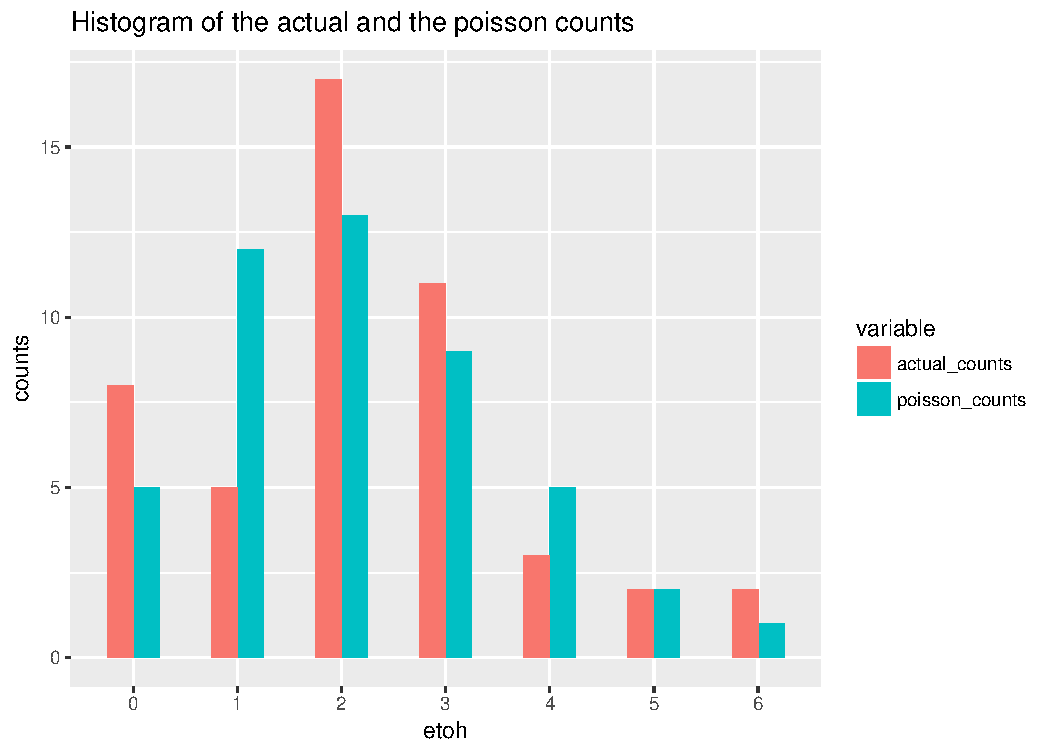
\includegraphics[width=\maxwidth]{figure/unnamed-chunk-3-1} 

\end{knitrout}

We see that the zeros in the actual counts are more than if the data had a poisson distribution. Due to this excess of zeros we would argue to use a hurdle model. 

\vspace{5mm}

We also present a table below to compare the actual counts and the counTs we would have obtained if the data followed a poisson distribution more closely. 

\vspace{7mm}

\begin{knitrout}
\definecolor{shadecolor}{rgb}{0.969, 0.969, 0.969}\color{fgcolor}
\begin{tabular}{l|r|r}
\hline
etoh & actual\_counts & poisson\_counts\\
\hline
0 & 8 & 5\\
\hline
1 & 5 & 12\\
\hline
2 & 17 & 13\\
\hline
3 & 11 & 9\\
\hline
4 & 3 & 5\\
\hline
5 & 2 & 2\\
\hline
6 & 2 & 1\\
\hline
\end{tabular}


\end{knitrout}


\vspace{5mm}

Clearly, as we have said before there are more zero in the data then a poisson distribution would have hence the data suggests that we should use a model whiCh incorporates this information into it. Also, we cannot do the Pearson Chi square goodness of fit test because more than 20\% of the events have expected frequencies below 5. If we ignore this access number of zeros we will be loosing a key characteristic of our data. It is important not to ignore this because if we assume the model has poisson distribution and infact it does not then we will be violating one of the assumptions of the model and our conclusions from the model may be end up being completely wrong.  


\vspace{5mm}


% Lastly, we will do a Vuong test to test if a poisson model is better or the model that in corporates the excess zeros called the hurdle model. 





\section*{Question 2}

Fit and interpret a hurdle model (with Poisson count distribution) for etoh that contains main effects of hx, ptsdsx, and affect. Do not include interaction terms in the model. Note, the pscl package in R contains a hurdle model fitting function. [12 points]

\vspace{5mm}

{\bf Answer:} Below we fit the specified hurdle model.

\begin{knitrout}
\definecolor{shadecolor}{rgb}{0.969, 0.969, 0.969}\color{fgcolor}\begin{kframe}
\begin{alltt}
\hlcom{## hurdle model}
\hlstd{model1} \hlkwb{<-} \hlkwd{hurdle}\hlstd{(}\hlkwc{formula} \hlstd{= etoh} \hlopt{~} \hlstd{hx} \hlopt{+} \hlstd{ptsdsx} \hlopt{+} \hlstd{affect,}
                             \hlkwc{dist}    \hlstd{=} \hlstr{"poisson"}\hlstd{,}
                             \hlkwc{data}    \hlstd{= daata)}
\hlkwd{summary}\hlstd{(model1)}
\end{alltt}
\begin{verbatim}
## 
## Call:
## hurdle(formula = etoh ~ hx + ptsdsx + affect, data = daata, dist = "poisson")
## 
## Pearson residuals:
##      Min       1Q   Median       3Q      Max 
## -2.13296 -0.70557 -0.09372  0.66604  2.04372 
## 
## Count model coefficients (truncated poisson with log link):
##             Estimate Std. Error z value Pr(>|z|)  
## (Intercept)   0.7685     0.3483   2.207   0.0273 *
## hx           -0.3811     0.2885  -1.321   0.1864  
## ptsdsx       -0.2974     0.1434  -2.073   0.0381 *
## affect        0.2457     0.1149   2.137   0.0326 *
## Zero hurdle model coefficients (binomial with logit link):
##             Estimate Std. Error z value Pr(>|z|)  
## (Intercept)   1.9799     1.4014   1.413   0.1577  
## hx           -2.2233     0.9122  -2.437   0.0148 *
## ptsdsx       -0.1978     0.4186  -0.473   0.6365  
## affect        0.3603     0.3565   1.011   0.3122  
## ---
## Signif. codes:  0 '***' 0.001 '**' 0.01 '*' 0.05 '.' 0.1 ' ' 1 
## 
## Number of iterations in BFGS optimization: 10 
## Log-likelihood: -77.44 on 8 Df
\end{verbatim}
\begin{alltt}
\hlstd{expCoef} \hlkwb{<-} \hlkwd{exp}\hlstd{(}\hlkwd{coef}\hlstd{((model1)))}
\hlstd{expCoef}
\end{alltt}
\begin{verbatim}
## count_(Intercept)          count_hx      count_ptsdsx      count_affect 
##         2.1565703         0.6830924         0.7427388         1.2784578 
##  zero_(Intercept)           zero_hx       zero_ptsdsx       zero_affect 
##         7.2420276         0.1082484         0.8205302         1.4337554
\end{verbatim}
\end{kframe}
\end{knitrout}

\subsection*{Interpreting the count model}

The average number of drinks a person has had in the last 24 hours is 2. This average number of drinks in the last 24 hours is increased by 1.3 times if a person's emotional state improves by one unit on the emotional state score. However, an increase in one unit of Post-Traumatic Stress Disorder severity score, decreases the average number of drinks (which is 2) a person had in the last 24 hours by 0.74 times. Both of these variables are statistically siginificant as their pvalues are less than 0.05 (pvalue = 0.0381 and pvalue = 0.0326 respectively). A person's history of alcohol abuse is not statistically significant ( pvalue = 0.1577 is greater than 0.05) meaning that it does not appear to effect the number of average drink he will have in the last 24 hours if he is an alcohol drinker. 

% The participant's Post-Traumatic Stress Disorder's degree of severity and the his emotional state over the previous 24 hours affect the number of drinks consumed by the him over the past 24 hours. An increase in one unit on the Post-Traumatic Stress Disorder severity score decreases the average number of drinks a person had in the past 24 hours by 0.74 (exp(-0.2974)) times. An increase in the emotional state of the participant by one unit on the emotional state score, keeping all else unchanged, increases the average number of drink consumed by a person in the last 24 hours by 1.3 (exp(0.2457)) times. 

\subsection*{Interpretation of the Zero-hurdle model}

The baseline odds of having drunk alcohol in the last 24 hours versus not having drunk any alcohol in the past 24 hours is 7.24. We can also consider this odds to be the odds of being an alcoholic or not being an alcoholic. This odds of drinking some alcohol versus not drinking any alcohol at all decreases by 0.10 times if the person has a history of alcohol abuse. And this effect is indeed statistically significant since pvalue = 0.015 is less than 0.05. The other variables do not have a statistically significant affect on if the person will drinking or not drink alcohol at all in the past 24 hours or in the other interpretation this means that, the other variables do not affect the odds of a person being alcoholic or not. 

\subsection*{General remarks}


Now one potential problem we could have is of multicolinearity. It is possible that the score indicating severity of PTSD symptoms experienced by the participant over the past 24 hours could be correlated with the score indicating the participant's emotional state over the previous 24 hours. From below we see that the two are mildly correlated (cor = 0.4606). Also, from the scatter plot we see that there is some underlying phenomena going on, which has sort of grouped the data points into two clusters. It is possible that these two clusters are two different types of people for example one could be males and others could be females or could be any sort of groups. Now within each cluster the severity of PTSD and the emotional state are negatively correlated. However, the overall correlation we obtained was positive. This is known as the Simpson's paradox and indicates that we should be very careful about the interpretation of our results especially the interpretation of how our variables are associated with one another since looking at the overall association between variables could be completely wrong and misleading and when we actually look at different groups of the data then the true relationship is revealed which could be very different from the overall one. A quick example would be that males and females when looked at seperately, both have a negative correlation between variables. However, looking at them together we get the completely incorrect relationship. Hence, I would suggest to be vary of our results of the hurdle model and accept that it is possible that our interpretations are not correct. We would need to do further group wise analysis on the data. 
\begin{knitrout}
\definecolor{shadecolor}{rgb}{0.969, 0.969, 0.969}\color{fgcolor}\begin{kframe}
\begin{alltt}
\hlkwd{plot}\hlstd{(daata}\hlopt{$}\hlstd{ptsdsx, daata}\hlopt{$}\hlstd{affect,} \hlkwc{xlab} \hlstd{=} \hlstr{"PTSD severity score"}\hlstd{,} \hlkwc{ylab} \hlstd{=} \hlstr{"Emotional State Score"}\hlstd{,} \hlkwc{main} \hlstd{=} \hlstr{"Correlation plot"}\hlstd{)} \hlcom{#daata$hx)}
\end{alltt}
\end{kframe}
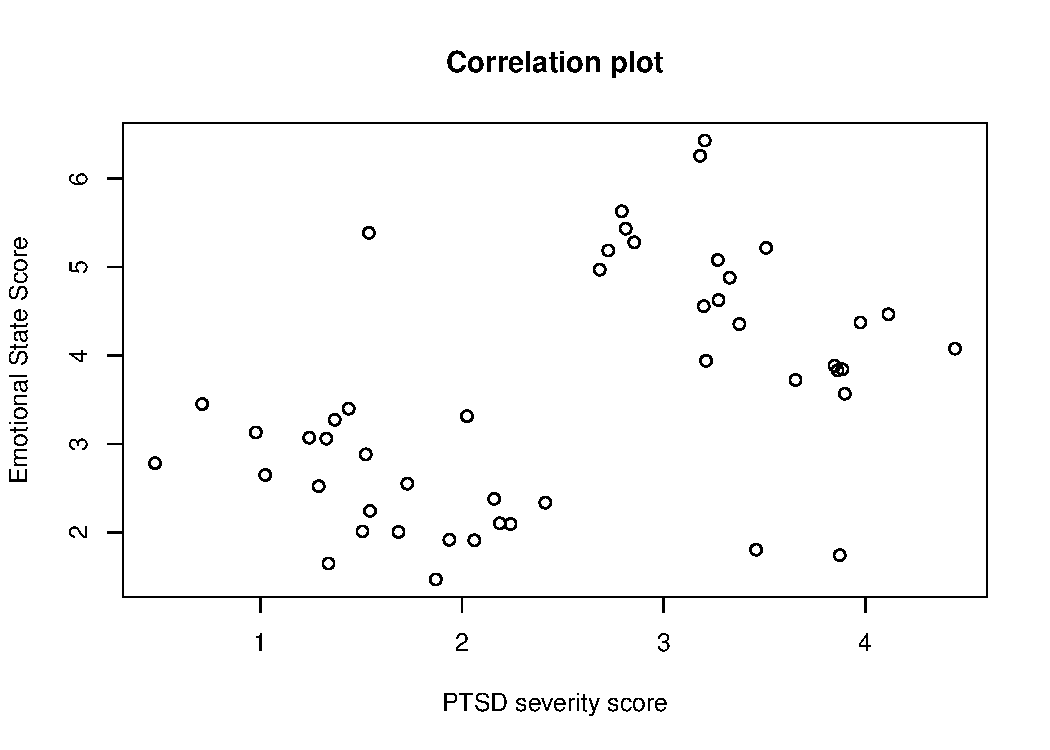
\includegraphics[width=\maxwidth]{figure/unnamed-chunk-7-1} 
\begin{kframe}\begin{alltt}
\hlkwd{cor}\hlstd{(daata}\hlopt{$}\hlstd{ptsdsx, daata}\hlopt{$}\hlstd{affect)}
\end{alltt}
\begin{verbatim}
## [1] 0.4606311
\end{verbatim}
\end{kframe}
\end{knitrout}



Note that this is an observational study as no experiment was conducted. Hence, it is very highly possible that there are other things outside a person's  PTSD score, their history of alcohol abuse and their emotional state over the previous 24 hours that could be impacting if a person drank alcohol at all in the past 24 hours or not and how many drinks he had. Such as if a person just  obtained some money in the last 24 hours then that could be the actual reason why he had those drinks or if the peson was with friends and because the friends were having drinks or not is why he had that many and the other variables of history of alcohol abuse, PTSD score, etc could be coincidentally, statistically significant in our study.  

\vspace{5mm}

Also some of the associations appear to be counter intutive. Such as having a history of alcohol abuse, causing a reduction in the odds of drinking alcohol in the past 24 hours. But it is not so counter intutive if you think about it a little. It is quite possible that those who have a history of alcohol abuse have had therapy and/or done rehab in the past hence are more likely to be able to control themselves and not drink any alcohol. Also, since this is an observational study, then there are many other things that could be affecting the number of drinks a person had in the last 24 hours and hence we causing the associations to appear not as straight forward as one would think. 


\section*{Question 3}

The investigator would like to know if any of these three explanatory variables
are superfluous. Please address this query. [4 points]

\vspace{5mm}

{\bf Answer:} It appears that the pearon's history of alcohol abuse does not impact the average number of drinks he has consumed in the past 24 hours as it is not statistically significant (p-value = 0.186, which is greater than 0.05) but it affect the odds of a person having drank alcohol or not at all in the past 24 hours as the p-value is greater than 0.05 (pvalue = 0.0148). Hence, this variable is not suprefluous.


\vspace{5mm}

Secondly, a person's emotional state in the past 24 hours does not affect if he would have drank alcohol or not at all in the past 24 hours, in other words, if he is an alcohol drinker or not (p-value = 0.6365, is greater than 0.05) nor does his Post-Traumatic Stress Disorder severity (p-value = 0.31 > 0.05) affect his odds of having drank alcohol or not at all in the past 24 hours.  His Post-Traumatic Stress Disorder's degree of severity and the his emotional state over the previous 24 hours affect the number of drinks consumed by the him over the past 24 hours as the p-values are greater than 0.05 (pvalues 0.0381 and 0.0326 respectively). Hence, again, neither of the two variables apear to be superfluous. In conclusion none of the variables are superfluous. 

% None of the explanatory variables appear to be superfluous because the participant's history of alcohol abuse impacts if he will drink any alchohol or not in the last 24 hours. His Post-Traumatic Stress Disorder's degree of severity and the his emotional state over the previous 24 hours affect the number of drinks consumed by the him over the past 24 hours. Hence, none of the variables appear to be superfluous. 

\section*{ Question 4} 

The investigator suggested that they have had an affinity for using a forward
selection model building approach that identifies, at each step, candidate
main-effect variables for which the Wald test has a p-value < 0.25. Apply
this model-building algorithm and describe the fitted final model. How does
interpretation of the associations differ between this fitted final model and the fitted model from Question 2 (above). Which model would you recommend as
a more appropriate representation of the data? [8 points]

\vspace{5mm}

{\bf Answer:} We demonstrate this forward selection model building approach below where we start with the model with no explanatory variables and only add one variable at a time and compare the two models using the Wald test, hence testing for the main effect of the added variable. 
 
 
 
\begin{knitrout}
\definecolor{shadecolor}{rgb}{0.969, 0.969, 0.969}\color{fgcolor}\begin{kframe}
\begin{alltt}
\hlcom{## hurdle model}

\hlstd{min.model} \hlkwb{=} \hlkwd{hurdle}\hlstd{(}\hlkwc{formula} \hlstd{= etoh} \hlopt{~} \hlnum{1}\hlstd{,} \hlkwc{dist} \hlstd{=} \hlstr{"poisson"}\hlstd{,} \hlkwc{data} \hlstd{= daata)}

\hlstd{mod0} \hlkwb{=} \hlkwd{hurdle}\hlstd{(}\hlkwc{formula} \hlstd{= etoh} \hlopt{~} \hlstd{hx,} \hlkwc{dist} \hlstd{=} \hlstr{"poisson"}\hlstd{,} \hlkwc{data} \hlstd{= daata)}

\hlkwd{waldtest}\hlstd{(min.model, mod0)}
\end{alltt}
\begin{verbatim}
## Wald test
## 
## Model 1: etoh ~ 1
## Model 2: etoh ~ hx
##   Res.Df Df  Chisq Pr(>Chisq)  
## 1     46                       
## 2     44  2 6.8358    0.03278 *
## ---
## Signif. codes:  0 '***' 0.001 '**' 0.01 '*' 0.05 '.' 0.1 ' ' 1
\end{verbatim}
\end{kframe}
\end{knitrout}

Since the p-value = 0.03278 is less than 0.25 we will include variable (hx) that indicates if a person had a history of alcohol abuse or not in the model. 

\vspace{5mm}

Now we will include the variable (ptsdsx) which is the score indicating severity of PTSD symptoms experienced by the participant over the past 24 hours into the model. 

\begin{knitrout}
\definecolor{shadecolor}{rgb}{0.969, 0.969, 0.969}\color{fgcolor}\begin{kframe}
\begin{alltt}
\hlcom{## hurdle model}

\hlstd{mod1} \hlkwb{=} \hlkwd{hurdle}\hlstd{(}\hlkwc{formula} \hlstd{= etoh} \hlopt{~} \hlstd{hx} \hlopt{+} \hlstd{ptsdsx,} \hlkwc{dist} \hlstd{=} \hlstr{"poisson"}\hlstd{,} \hlkwc{data} \hlstd{= daata)}

\hlkwd{waldtest}\hlstd{(mod0, mod1)}
\end{alltt}
\begin{verbatim}
## Wald test
## 
## Model 1: etoh ~ hx
## Model 2: etoh ~ hx + ptsdsx
##   Res.Df Df  Chisq Pr(>Chisq)
## 1     44                     
## 2     42  2 1.0604     0.5885
\end{verbatim}
\end{kframe}
\end{knitrout}

For this new variable since its pvalue 0.5885 is greater than 0.25 we will not inlcude it in the model. 

\vspace{5mm}

Lastly, we will include the score variable indicating the participants emotional state over the previous 24 hours to the model with the person's history of alcohol abuse. 

\begin{knitrout}
\definecolor{shadecolor}{rgb}{0.969, 0.969, 0.969}\color{fgcolor}\begin{kframe}
\begin{alltt}
\hlcom{## hurdle model}

\hlstd{mod2} \hlkwb{=} \hlkwd{hurdle}\hlstd{(}\hlkwc{formula} \hlstd{= etoh} \hlopt{~} \hlstd{hx} \hlopt{+} \hlstd{affect,} \hlkwc{dist} \hlstd{=} \hlstr{"poisson"}\hlstd{,} \hlkwc{data} \hlstd{= daata)}

\hlkwd{waldtest}\hlstd{(mod0, mod2)}
\end{alltt}
\begin{verbatim}
## Wald test
## 
## Model 1: etoh ~ hx
## Model 2: etoh ~ hx + affect
##   Res.Df Df  Chisq Pr(>Chisq)
## 1     44                     
## 2     42  2 1.8744     0.3917
\end{verbatim}
\end{kframe}
\end{knitrout}

Again since the pvalue 0.39 is greater than 0.25 we will not inlcude it in the model. Hence, the final model that we obtain is the hurdle model with only the histroy of alcohol abuse as the explanatory variable. 


\begin{knitrout}
\definecolor{shadecolor}{rgb}{0.969, 0.969, 0.969}\color{fgcolor}\begin{kframe}
\begin{alltt}
\hlkwd{summary}\hlstd{(mod0)}
\end{alltt}
\begin{verbatim}
## 
## Call:
## hurdle(formula = etoh ~ hx, data = daata, dist = "poisson")
## 
## Pearson residuals:
##     Min      1Q  Median      3Q     Max 
## -1.6462 -0.3769 -0.3352  0.3773  2.1619 
## 
## Count model coefficients (truncated poisson with log link):
##             Estimate Std. Error z value Pr(>|z|)    
## (Intercept)   0.9364     0.1240   7.555  4.2e-14 ***
## hx           -0.2515     0.2810  -0.895    0.371    
## Zero hurdle model coefficients (binomial with logit link):
##             Estimate Std. Error z value Pr(>|z|)    
## (Intercept)   2.7081     0.7303   3.708 0.000209 ***
## hx           -2.1972     0.8944  -2.457 0.014027 *  
## ---
## Signif. codes:  0 '***' 0.001 '**' 0.01 '*' 0.05 '.' 0.1 ' ' 1 
## 
## Number of iterations in BFGS optimization: 7 
## Log-likelihood: -80.8 on 4 Df
\end{verbatim}
\begin{alltt}
\hlkwd{exp}\hlstd{(}\hlkwd{coef}\hlstd{(mod0))}  \hlcom{# Exp of Coefficients of the forward stepwise model selectio. }
\end{alltt}
\begin{verbatim}
## count_(Intercept)          count_hx  zero_(Intercept)           zero_hx 
##         2.5508239         0.7776298        15.0000000         0.1111111
\end{verbatim}
\begin{alltt}
\hlkwd{exp}\hlstd{(}\hlkwd{coef}\hlstd{(model1))}  \hlcom{# Exp of Coefficients of the full model used in question 2}
\end{alltt}
\begin{verbatim}
## count_(Intercept)          count_hx      count_ptsdsx      count_affect 
##         2.1565703         0.6830924         0.7427388         1.2784578 
##  zero_(Intercept)           zero_hx       zero_ptsdsx       zero_affect 
##         7.2420276         0.1082484         0.8205302         1.4337554
\end{verbatim}
\end{kframe}
\end{knitrout}


{\bf Answer: }     The fitted final model is the hurdle model where only the  person's history of alcohol abuse or not is included. The model says that the average number of drinks a person has had in the past 24 hours is 2.55 and that this is not affected by if he had a histroy of alcohol abuse or not as the pvalue 0.371 is less than 0.05. Further, the model says that the basline odds of drinking alcohol in the past 24 hours versus not drinking any alcohol at all in the past 24 hours is 15. This odds is decreased by 0.11 times if the person had a history of alcohol abuse. 

\vspace{5mm}

The interpretation of the association between if a person had a history of alcohol abuse or not and the odds of drinking any alcohol or not and the average number of drinks a person had in the last 24 hours, both are the same in the two models. However, in the model using forward selection the model says that the  severity of PTSD symptoms experienced by the participant over the past 24 hours and  score indicating the participantants emotional state over the previous 24 hours have no effect on the average number of drinks a person had in the last 24 hours. This is because both of these variable are not present in the model. Which is different from the previous model which did say the both these variables affected the average number of drinks a person had in the last 24 hours. One other major difference between the two models is that the full model says that the baseline of someone drinking alcohol versus not drinking any alcohol in the last 24 hours is 7.24, whereas the baseline odds for the model from the stepwise forward selection is 15.0 which is almost double.  

\begin{knitrout}
\definecolor{shadecolor}{rgb}{0.969, 0.969, 0.969}\color{fgcolor}\begin{kframe}
\begin{alltt}
\hlstd{hx_model} \hlkwb{=} \hlkwd{round}\hlstd{(}\hlkwd{colSums}\hlstd{(}\hlkwd{predict}\hlstd{(mod0,} \hlkwc{type} \hlstd{=} \hlstr{"prob"}\hlstd{)[,}\hlnum{1}\hlopt{:}\hlnum{7}\hlstd{]),} \hlnum{0}\hlstd{)}
\hlstd{full_model} \hlkwb{=} \hlkwd{round}\hlstd{(}\hlkwd{colSums}\hlstd{(}\hlkwd{predict}\hlstd{(model1,} \hlkwc{type} \hlstd{=} \hlstr{"prob"}\hlstd{)[,}\hlnum{1}\hlopt{:}\hlnum{7}\hlstd{]),} \hlnum{0}\hlstd{)}
\hlstd{actual_counts} \hlkwb{=} \hlkwd{table}\hlstd{(daata}\hlopt{$}\hlstd{etoh)}

\hlkwd{kable}\hlstd{(}\hlkwd{rbind}\hlstd{(hx_model, full_model, actual_counts))}
\end{alltt}
\end{kframe}
\begin{tabular}{l|r|r|r|r|r|r|r}
\hline
  & 0 & 1 & 2 & 3 & 4 & 5 & 6\\
\hline
hx\_model & 8 & 10 & 11 & 9 & 6 & 3 & 1\\
\hline
full\_model & 8 & 11 & 11 & 8 & 5 & 3 & 1\\
\hline
actual\_counts & 8 & 5 & 17 & 11 & 3 & 2 & 2\\
\hline
\end{tabular}


\end{knitrout}

\vspace{5mm}


From the above table we see that both models are equally similar to the actual counts. No one model does particularly better than the other. However, when we include the other two characteristics as in the full model, we find that they have a statistically significant affect on the average number of drink a person has had in the last 24 hours (as the pvalues are greater than 0.05). Hence, they do explain the data and are a better representation of the data.

\vspace{5mm}


Secondly, since the goal of the study is to examine patient characteristics associated with self-medication through alcohol consumption. Where the characteristics are the three we have been mentioning so far. I would recommend using the model from question 2, which we have called the full model. This is because since the goal is to exam these characteristics then and since in the full model none of the characteristics appear to he superfluous then they should be inlcuded in the model. Our model also allows us to personalize the average number of drinks a person has had in the last 24 hours based on their other two characteristics. Hence, the full model represents the data better.

\vspace{5mm}

Lastly, I would not recommend using the model with only the person's history of alcohol abuse because it was obtained using stepwise forward model selection and I would highly advocate aginst using any stepwise forward model selection method. This is because using stepwise forward model selection we are doing multiple tests one after the other and then we find ourselves in the well known problem of multiple testing. Which basically is doing several statistical tests of significance at the same time or one after the other and then cherry picking the one which appears to be statistically significant (pvalue less than 0.05). One of the big problems of this is that the p-values no longer have the proper meaning and the chance of finding some test to be statistically significant just based on pure luck becomes much larger (type I error rate increases). Also, this is like cherry picking the results we want to show and not showing those we do not. It is also possible, that something which is, infact significant in explaning the model might not end up being in the model simply because of the order in which and how the variables were add to the model and we might miss very important variable because of this. Lastly, it also possible that our estimates are biased (it gives biased regression coefficients see Tibshirani [1996]).


\section*{Question 5}

The investigator is curious about the use of a hurdle model to accommodate
excess zeros. Explain the difference between hurdle and zero-inflated models.
Explain what you need to know about this study in order for you and the
investigator to decide whether the hurdle or zero-inflated model is more
appropriate for this study. [8 points]

\vspace{5mm}

{\bf Answer:}  In a hurdle model it is assumed that all the zeros come from a single source. In our example that means that all those participants that have had zero drinks in the past 24 hours comes from all the participants who are non-alcohol users or at least non-alcohol abusers. Hence, it is assumed that if you have a non-zero number of drinks you had in the past 24 hours then you have "passed the hurdle" of being a non-alcohol user. Therefore, in a hurdle model it is assumed that when one is modeling the number of zeros, one is in fact modeling the number of non-alcohol users. 

\vspace{5mm}

In the zero-inflated model it is assumed that the zeros come from two different sources. The first would be those who had no choice in the first place, for example could not drink alcohol because had no access to it. We call these people not-at-risk population and the zeros coming from these people, structural zeros. The second would be those who had the option of drinking alcohol but chose, by their own will, not to drink alcohol. These people we call at-risk population and the zeros coming from this population we call sampled zeros or actual zeros. Distinguishing these two types of zeros is very important because someone who did not drink alcohol because he had no access to it, and might have had if he had access to it, is inherently very different from someone who did not drink it by chioce. If this distinction is not made then the important characteristics of those who did not drink by choice could be confounded or mixed up with the characteristics of those who did not drink simply because of a lack of access to alcohol. Zero-inflated models take into account these two different types of zero counts in the model. 


\vspace{5mm}

Now, the fundamental difference between the two models is how they treat the zero counts. In hurdle model it is assumed that the zeros come from a single source (all of the zeroes are coming from the at-risk people and there are no people who are not-at-risk) and in the zero-inflated model it is assumed the zeros are produced due to two sources (at-risk people and not at rik people). Hence, to decide whether the hurdle or zero-inflated model is more appropriate for this study, we would need to identify what produces the zero counts and the type of zeros they are, i.e. if there are any structural zeros. And the main guidence to answering the question would come from looking at the design of the study so we can identify if there are any of these structural zeros. 

\vspace{5mm}

Therefore, if everyone had access to alcohol and everyone drinks or does not drink alcohol (is alcoholic or not) by choice then a hurdle model would be appropriate. However, if some people did have access to alcohol while others did not, implying there are structural zeros then the zero-inflated model will be more appropriate to use. Hence, we would need to know if there are any structural zeros in the study to decide which model to use. 


 

\end{document}
